\PassOptionsToPackage{unicode=true}{hyperref} % options for packages loaded elsewhere
\PassOptionsToPackage{hyphens}{url}
%
\documentclass[
  american,
  ignorenonframetext,
]{beamer}
\usepackage{pgfpages}
\setbeamertemplate{caption}[numbered]
\setbeamertemplate{caption label separator}{: }
\setbeamercolor{caption name}{fg=normal text.fg}
\beamertemplatenavigationsymbolsempty
\setbeameroption{hide notes}
% Prevent slide breaks in the middle of a paragraph:
\widowpenalties 1 10000
\raggedbottom
\usepackage{lmodern}
\usepackage{amssymb,amsmath}
\usepackage{ifxetex,ifluatex}
\ifnum 0\ifxetex 1\fi\ifluatex 1\fi=0 % if pdftex
  \usepackage[T1]{fontenc}
  \usepackage[utf8]{inputenc}
  \usepackage{textcomp} % provides euro and other symbols
\else % if luatex or xelatex
  \usepackage{unicode-math}
  \defaultfontfeatures{Scale=MatchLowercase}
  \defaultfontfeatures[\rmfamily]{Ligatures=TeX,Scale=1}
\fi
\usetheme[]{UOS}
% use upquote if available, for straight quotes in verbatim environments
\IfFileExists{upquote.sty}{\usepackage{upquote}}{}
\IfFileExists{microtype.sty}{% use microtype if available
  \usepackage[]{microtype}
  \UseMicrotypeSet[protrusion]{basicmath} % disable protrusion for tt fonts
}{}
\makeatletter
\@ifundefined{KOMAClassName}{% if non-KOMA class
  \IfFileExists{parskip.sty}{%
    \usepackage{parskip}
  }{% else
    \setlength{\parindent}{0pt}
    \setlength{\parskip}{6pt plus 2pt minus 1pt}}
}{% if KOMA class
  \KOMAoptions{parskip=half}}
\makeatother
\usepackage{xcolor}
\IfFileExists{xurl.sty}{\usepackage{xurl}}{} % add URL line breaks if available
\IfFileExists{bookmark.sty}{\usepackage{bookmark}}{\usepackage{hyperref}}
\hypersetup{
  pdftitle={File Input/Ouput},
  pdfauthor={Julia Wippermann; Robin Horn; Kamran Vatankhah-Barazandeh; Leonard Frommelt},
  pdfborder={0 0 0},
  breaklinks=true}
\urlstyle{same}  % don't use monospace font for urls
\newif\ifbibliography
\usepackage{listings}
\newcommand{\passthrough}[1]{#1}
\lstset{defaultdialect=[5.3]Lua}
\lstset{defaultdialect=[x86masm]Assembler}
\usepackage{longtable,booktabs}
\usepackage{caption}
% These lines are needed to make table captions work with longtable:
\makeatletter
\def\fnum@table{\tablename~\thetable}
\makeatother
\usepackage{graphicx,grffile}
\makeatletter
\def\maxwidth{\ifdim\Gin@nat@width>\linewidth\linewidth\else\Gin@nat@width\fi}
\def\maxheight{\ifdim\Gin@nat@height>\textheight\textheight\else\Gin@nat@height\fi}
\makeatother
% Scale images if necessary, so that they will not overflow the page
% margins by default, and it is still possible to overwrite the defaults
% using explicit options in \includegraphics[width, height, ...]{}
\setkeys{Gin}{width=\maxwidth,height=\maxheight,keepaspectratio}
\setlength{\emergencystretch}{3em}  % prevent overfull lines
\providecommand{\tightlist}{%
  \setlength{\itemsep}{0pt}\setlength{\parskip}{0pt}}
\setcounter{secnumdepth}{-2}

% set default figure placement to htbp
\makeatletter
\def\fps@figure{htbp}
\makeatother

\usepackage{minted}
\newminted{python}{linenos=false}
\newminted[outputcode]{text}{frame=single, framesep=5pt}
\newenvironment{pyexec}[1]{\noindent \textbf{Output: }  #1}{}
\ifnum 0\ifxetex 1\fi=0 % if pdftex or luatex
  \usepackage[shorthands=off,main=american]{babel}
\else % if xetex
  % load polyglossia as late as possible as it *could* call bidi if RTL lang (e.g. Hebrew or Arabic)
  \usepackage{polyglossia}
  \setmainlanguage[variant=american]{english}
\fi

\title{File Input/Ouput}
\author[J.~Wip., R.~Horn, K.~Vat.-Bar., L.~Fro.]{Julia Wippermann \and Robin Horn \and Kamran Vatankhah-Barazandeh \and Leonard Frommelt}
\date{May 17, 2021}

\begin{document}
\frame[plain]{\titlepage}

\begin{frame}
  \tableofcontents[hideallsubsections]
\end{frame}
\hypertarget{recap}{%
\section{Recap}\label{recap}}

\begin{frame}[fragile,fragile]{General Tips}
\protect\hypertarget{general-tips}{}

\begin{itemize}
\item
  submit executable code
\item
  read the error messages
\item
  have a look at the corrections
\end{itemize}

\note{Try to make your code runnable. It's okay if there are logical
errors, but you are able to read and fix SyntaxErrors since the second
lecture. You will not get more than 50\% of the points for a task if
your code cannot be executed. This will be handled more strictly every
week. In the last week you will not get more than 25\% of the points for
a task if your code cannot be executed.}

\end{frame}

\begin{frame}[fragile,fragile]{Recap: print() revisited}
\protect\hypertarget{recap-print-revisited}{}

\begin{pythoncode}

print(1, 2, 3, 4, sep='*')
print(1, 2, 3, 4, sep='#', end='&')

\end{pythoncode}

\begin{pyexec}

\begin{outputcode}

1*2*3*4
1#2#3#4&

\end{outputcode}

\end{pyexec}

\note{The \texttt{sep} argument is by default space for the
\texttt{print()} function. In this case we set it to \texttt{*} or
\texttt{\#}.}

\end{frame}

\begin{frame}[fragile,fragile]{Recap: String Operations}
\protect\hypertarget{recap-string-operations}{}

\begin{pythoncode}

text = "Lara Meier\nAnna Müller\nJana Schmidt"
print(text)

\end{pythoncode}

\begin{pyexec}

\begin{outputcode}

Lara Meier
Anna Müller
Jana Schmidt

\end{outputcode}

\end{pyexec}

\end{frame}

\begin{frame}[fragile,fragile]{Recap: split()}
\protect\hypertarget{recap-split}{}

\begin{pythoncode}

text = "Lara Meier\nAnna Müller\nJana Schmidt"

# split between each first and last name
names = text.split()
print(names)

\end{pythoncode}

\begin{pyexec}

\begin{outputcode}

['Lara', 'Meier', 'Anna', 'Müller', 'Jana',
'Schmidt']

\end{outputcode}

\end{pyexec}

\note{\texttt{split()}: splits a string into a list of strings (by
default it splits at whitespace).}

\end{frame}

\begin{frame}[fragile,fragile]{Recap: splitlines()}
\protect\hypertarget{recap-splitlines}{}

\begin{pythoncode}

text = "Lara Meier\nAnna Müller\nJana Schmidt"

# splits between each name
names = text.splitlines()
print(names)

\end{pythoncode}

\begin{pyexec}

\begin{outputcode}

['Lara Meier', 'Anna Müller', 'Jana Schmidt']

\end{outputcode}

\end{pyexec}

\note{\texttt{splitlines()}: splits a string at each line break into a
list of strings.}

\end{frame}

\hypertarget{io-streams}{%
\section{I/O Streams}\label{io-streams}}

\begin{frame}[fragile,fragile]{By the end of this lecture you will know
how to \ldots{}}
\protect\hypertarget{by-the-end-of-this-lecture-you-will-know-how-to}{}

\begin{itemize}
\item
  read in text files
\item
  write to text files
\item
  work with \texttt{csv} files
\end{itemize}

\note{\begin{itemize}
\tightlist
\item
  csv stands for comma separated values (more about this later)
\end{itemize}}

\end{frame}

\begin{frame}[fragile,fragile]{Kinds of Files}
\protect\hypertarget{kinds-of-files}{}

\textbf{Text files}

\begin{itemize}
\tightlist
\item
  made of readable text characters \vspace{1.5em}
\end{itemize}

\textbf{Binary files}

\begin{itemize}
\tightlist
\item
  contain unformatted data, saved in its raw memory format
\end{itemize}

\note{\textbf{Binary files}

contain unformatted data, saved in its raw memory format. They are
computer- but not human-readable. For example, the integers 1, 351,
473829 are all stored as 4 or 8 byte integers while their string
representations would be 1, 3 and 6 byte values. The details are not
important for this course.}

\end{frame}

\begin{frame}[fragile,fragile]{Keyboard Input}
\protect\hypertarget{keyboard-input}{}

\begin{itemize}
\tightlist
\item
  keyboard input is nice to interact with the user
\end{itemize}

\texttt{answer\ =\ input("What\ is\ your\ name?\ ")} \vspace{2em}

\textbf{But how to work with a lot of data?}

\(\rightarrow\) you will need to read data from files and save data to
files

\end{frame}

\begin{frame}[fragile,fragile]{Why do we need to learn how to work with
files?}
\protect\hypertarget{why-do-we-need-to-learn-how-to-work-with-files}{}

\begin{itemize}
\item
  to handle large amount of data
\item
  to export data from a database
\item
  to use data as input to another program
\end{itemize}

\note{For example:

\begin{itemize}
\item
  conducting an experiment (storing the records of the participants)
\item
  downloading data sets
\end{itemize}}

\end{frame}

\begin{frame}[fragile,fragile]{Input Output Streams}
\protect\hypertarget{input-output-streams}{}

\begin{itemize}
\tightlist
\item
  I/O stands for \emph{Input and Output}
\end{itemize}

\note{We already got to know an output stream:

The standard output stream (\texttt{stout})

\begin{itemize}
\item
  we use the \texttt{print()} function to output data to the standard
  output device (screen)
\item
  we can also use the print function to write data to a file (will be
  discussed later)
\end{itemize}}

\end{frame}

\begin{frame}[fragile,fragile]{Streams}
\protect\hypertarget{streams}{}

``In~computer science, a~stream~is a~sequence~of~data elements~made
available over time''

Wikipedia (2018) \vspace{1em}

\begin{itemize}
\item
  \texttt{stdin}
\item
  \texttt{stdout}
\item
  \texttt{stderr}
\end{itemize}

\note{A stream can be thought of as items on a conveyor belt being
processed one at a time rather than in large batches (Wikipedia (2018)).
There are three standard streams that are supported by most programming
languages and connect the program~with its environment:

\begin{itemize}
\tightlist
\item
  \textbf{Standard input stream (\texttt{stdin})}

  \begin{itemize}
  \tightlist
  \item
    leads~data into an application
  \item
    usually this data comes from~the keyboard~or other hardware
  \end{itemize}
\item
  \textbf{Standard output stream (\texttt{stdout})}

  \begin{itemize}
  \tightlist
  \item
    leads data out of an application
  \item
    usually to the terminal
  \end{itemize}
\item
  \textbf{Standard error stream (\texttt{stderr})}

  \begin{itemize}
  \tightlist
  \item
    leads error-/diagnostics data out of an application
  \item
    usually this also goes to the terminal
  \end{itemize}
\end{itemize}}

\end{frame}

\begin{frame}[fragile,fragile]{Standard Output Stream}
\protect\hypertarget{standard-output-stream}{}

\begin{pythoncode}

import sys

print(*objects, sep=' ', end='\n', file=sys.stdout)

\end{pythoncode}

Have a look at the Python 3 Documentation
\href{https://docs.python.org/3/library/functions.html\#print}{\textbf{here}}.

\note{\texttt{print(*objects,\ sep=\textquotesingle{}\ \textquotesingle{},\ end=\textquotesingle{}\textbackslash{}n\textquotesingle{},\ file=sys.stdout)}
\vspace{1em}

With the \texttt{print()} function, you print objects

\quad \quad to the stream \texttt{file},

\quad \quad separated by \texttt{sep}

\quad \quad and followed by \texttt{end}. \vspace{1em}

\texttt{sep}, \texttt{end} and \texttt{file} must be given as keyword
arguments. \vspace{2em}}

\end{frame}

\hypertarget{opening-and-closing-a-file}{%
\section{Opening and Closing a File}\label{opening-and-closing-a-file}}

\begin{frame}[fragile,fragile]{Opening, Printing to and Closing a File}
\protect\hypertarget{opening-printing-to-and-closing-a-file}{}

\begin{pythoncode}

# initializing my lottery numbers
numbers = [21, 8, 19, 9, 1, 22]

# opening the file in write mode
lottery_file = open('lottery.txt', 'w')
# printing data to the file
print(numbers, file=lottery_file)
# closing the file
lottery_file.close()

\end{pythoncode}

\begin{pyexec}

\begin{outputcode}

\end{outputcode}

\end{pyexec}

\note{After~opening a file, you can~use~\texttt{print()} with the file
as a keyword argument to~write to the file. Opening a file technically
means~creating a stream such that data~is able to flow from the file to
the application or vice versa.

Files that are opened need to be closed after use. The data stream needs
to be closed down to~confirm~that no more data~will be transferred, to
free up resources that were made available for the stream, and to make
the file accessible for other processes.}

\end{frame}

\begin{frame}[fragile,fragile]{}
\protect\hypertarget{section}{}

\begin{pythoncode}

# initializing my lottery numbers
numbers = [21, 8, 19, 9, 1, 22]

# taking care of opening and closing
with open('lottery.txt', 'w') as lottery_file:
    # printing data to the file
    print(numbers, file=lottery_file)

\end{pythoncode}

\note{There is another notation that makes the opening \textbf{and}
closing of files easier: using a \textbf{\texttt{with}} statement.

The \texttt{with}~statement calls a context manager. The context manager
handles the opening and closing of the file for you. Using this notation
is heavily recommended and common practice.

We recommend~that you~only use \texttt{open()} and \texttt{close()}
manually if~you cannot do it otherwise.

\textbf{Pathvariables:} You can always assume we have the files in the
same directory as the scripts (unless otherwise mentioned), so just use
the filenames.}

\end{frame}

\begin{frame}[fragile,fragile]{Writing to a File}
\protect\hypertarget{writing-to-a-file}{}

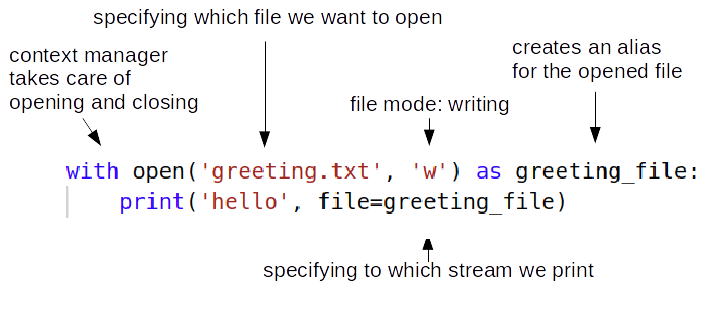
\includegraphics[width=1\textwidth,height=\textheight]{06_FileIO/with_open_annotated.png}

\end{frame}

\begin{frame}[fragile,fragile]{File Modes}
\protect\hypertarget{file-modes}{}

\begin{longtable}[]{@{}ll@{}}
\toprule
Mode & Description\tabularnewline
\midrule
\endhead
r & To read a file (default)\tabularnewline
w & To write a file; Creates a new file if it doesn't
exist\tabularnewline
a & To append at the end of file; create if doesn't exist\tabularnewline
+ & To open a file for updating (reading or writing)\tabularnewline
\bottomrule
\end{longtable}

\note{File modes: the letter after the \texttt{file\ name} is the mode.
It can be one of:

\begin{itemize}
\item
  \texttt{w} write (overwrites/creates)
\item
  \texttt{r} read (read-only)
\item
  \texttt{a} append (updates/creates)
\item
  add \texttt{+} to open for read and write (e.g.~\texttt{r+})
\item
  some more that we are not going to cover in this lecture
\end{itemize}}

\end{frame}

\begin{frame}[fragile,fragile]{File Modes}
\protect\hypertarget{file-modes-1}{}

\begin{figure}
\centering
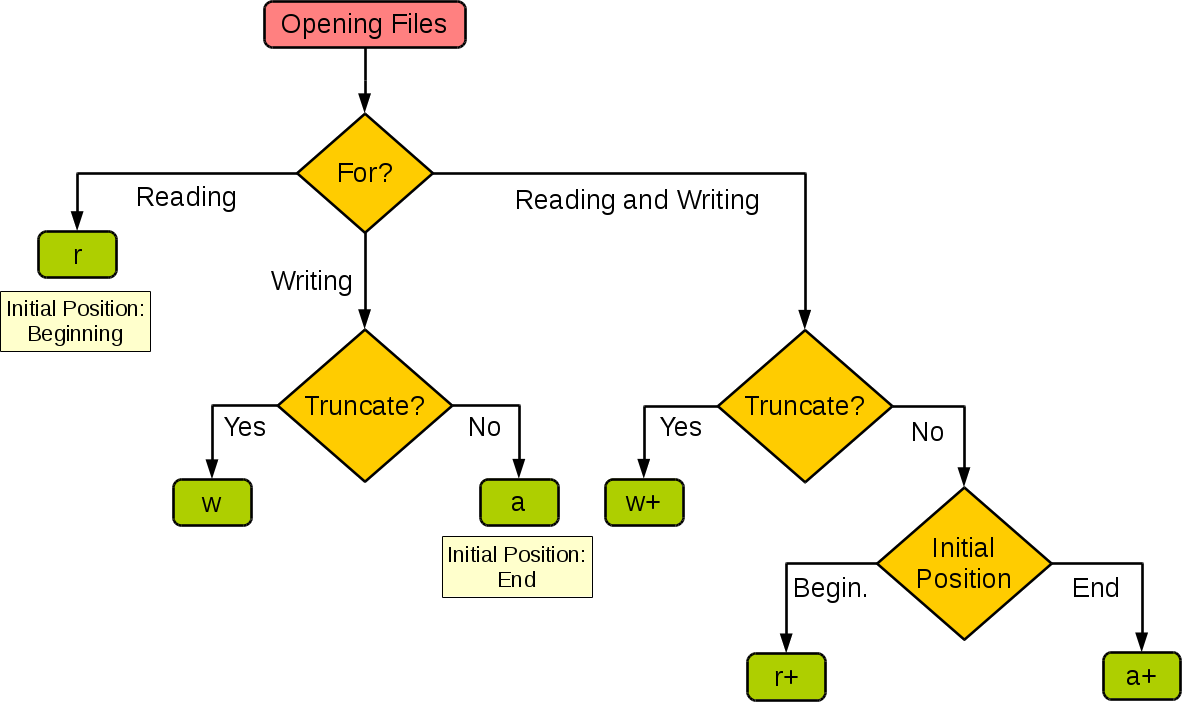
\includegraphics[width=0.9\textwidth,height=\textheight]{06_FileIO/read_write_mode.png}
\caption{https://stackoverflow.com/a/30566011}
\end{figure}

\note{\begin{itemize}
\item
  opening a file for reading should be done with mode \texttt{r}.
\item
  if you open a file with \texttt{w}, it is cleared.
\item
  if you want to avoid clearing but still write, use \texttt{a} for
  appending
\item
  or, if you want read and write, use \texttt{r+}
\end{itemize}}

\end{frame}

\hypertarget{reading-from-and-writing-to-a-file}{%
\section{Reading from and Writing to a
File}\label{reading-from-and-writing-to-a-file}}

\begin{frame}[fragile,fragile]{Reading in Data from a File}
\protect\hypertarget{reading-in-data-from-a-file}{}

\begin{pythoncode}

# taking care of opening and closing (file mode: read)
with open('greeting.txt', 'r') as greet_file:
    print(greet_file.read())

\end{pythoncode}

\begin{pyexec}

\begin{outputcode}

hello

\end{outputcode}

\end{pyexec}

\note{The code works given the file \texttt{greeting.txt} (like the one
we created on previous slides) exists. \vspace{1em}

To read from a file we use \texttt{read()}.

When we give \texttt{read()} an argument i.e.~\texttt{read(n)}, we only
read the first \texttt{n} characters. For example \texttt{read(5)} reads
the first 5 characters.}

\end{frame}

\begin{frame}[fragile,fragile]{Writing to a File}
\protect\hypertarget{writing-to-a-file-1}{}

\begin{pythoncode}

text = "Lara Meier\nAnna Müller\nJana Schmidt"

with open('names.txt', 'w') as name_file:
    # writing the names to a file
    name_file.write(text)

\end{pythoncode}

\begin{pyexec}

\begin{outputcode}

\end{outputcode}

\end{pyexec}

\note{To write to a file we use \texttt{write()} and give it the string,
that we want to write to the file, as an argument.

In this example, we open the file in
\texttt{\textquotesingle{}w\textquotesingle{}} mode. If a file with the
name \texttt{names.txt} does not exist yet, a new one is created and we
write the \texttt{text} string into it. If the file \texttt{names.txt}
did exist beforehand, the file \texttt{names.txt} is cleared and we
write the \texttt{text} string into it. As we do not direct any data to
the standard output stream, there is nothing displayed on the terminal.}

\end{frame}

\begin{frame}[fragile,fragile]{Reading a File Line by Line}
\protect\hypertarget{reading-a-file-line-by-line}{}

\begin{pythoncode}

# taking care of opening and closing (file mode: read)
with open('names.txt', 'r') as names_file:
    # make a list of each line of the file
    name_records = names_file.read().splitlines()
    for line in name_records:
        print(line)

\end{pythoncode}

\begin{pyexec}

\begin{outputcode}

Lara Meier
Anna Müller
Jana Schmidt

\end{outputcode}

\end{pyexec}

\note{The code works given the file \texttt{names.txt} (like the one we
created on previous slides) exists. \vspace{1em}

In this example, we want to print the names from the file to the
terminal.}

\end{frame}

\begin{frame}[fragile,fragile]{Reading a File Line by Line}
\protect\hypertarget{reading-a-file-line-by-line-1}{}

\begin{pythoncode}

# we want to have a list of the last names

with open('names.txt', 'r') as names_file:
    lastnames = []
    for name in names_file:
        first_and_last = name.split()
        lastnames.append(first_and_last[1])
    print(lastnames)

\end{pythoncode}

\begin{pyexec}

\begin{outputcode}

['Meier', 'Müller', 'Schmidt']

\end{outputcode}

\end{pyexec}

\note{The code works given the file \texttt{names.txt} (like the one we
created on previous slides) exists. \vspace{1em}

We want to make a list of the last names that we find in the file
\texttt{names.txt}.

The code shows that you can also iterate over a file line by line.}

\end{frame}

\begin{frame}[fragile,fragile]{Where does reading a file begin?}
\protect\hypertarget{where-does-reading-a-file-begin}{}

\begin{pythoncode}

with open('names.txt', 'r') as names_file:
    names = names_file.read().splitlines()
    names_again = names_file.read().splitlines()

print(names)
print(names_again)

\end{pythoncode}

\begin{pyexec}

\begin{outputcode}

['Lara Meier', 'Anna Müller', 'Jana Schmidt']
[]

\end{outputcode}

\end{pyexec}

\note{The code works given the file \texttt{names.txt} (like the one we
created on previous slides) exists. \vspace{1em}

The code shows that you have to keep in mind where you begin reading a
file and until which point you already read the data. You can use
\texttt{seek} to have more control about this (which will not be covered
further in the lecture). Have a look at the diagram on slide 21 to learn
more about this. The position where you begin reading depends on the
file mode in which you open the file.}

\end{frame}

\begin{frame}[fragile,fragile]{Writing Data to a File}
\protect\hypertarget{writing-data-to-a-file}{}

\begin{pythoncode}

# list of lottery numbers
numbers = [21, 8, 19, 9, 1, 22]

with open('lottery.txt', 'w') as lottery_file:
    lottery_file.write(numbers)

\end{pythoncode}

\begin{pyexec}

\begin{outputcode}

Traceback (most recent call last):
  File "<string>", line 5, in <module>
TypeError: write() argument must be str, not list

\end{outputcode}

\end{pyexec}

What do we learn from this?

\note{In this example, we want to write the \texttt{list} of lottery
numbers to the file. From the error message, we learn that the argument
that we pass to the function \texttt{write()} needs to be a string.

Ok, so let's correct that!}

\end{frame}

\begin{frame}[fragile,fragile]{Writing Data to a File}
\protect\hypertarget{writing-data-to-a-file-1}{}

\begin{pythoncode}

numbers = [21, 8, 19, 9, 1, 22]

with open('lottery.txt', 'w') as lottery_file:
    # we cast the number list into a str
    lottery_file.write(str(numbers))

with open('lottery.txt', 'r') as lottery_file:
    result = lottery_file.read()
    print(result, type(result))

\end{pythoncode}

\begin{pyexec}

\begin{outputcode}

[21, 8, 19, 9, 1, 22] <class 'str'>

\end{outputcode}

\end{pyexec}

\note{Great! Writing the list of lottery numbers to the file worked.

By looking at the output, we also find out that when we use
\texttt{read()} to read in the data from a file, we get a string back.

But of course we want to continue working with a \texttt{list}.}

\end{frame}

\begin{frame}[fragile,fragile]{There are only Strings \ldots{}}
\protect\hypertarget{there-are-only-strings}{}

\begin{pythoncode}

>>> b = "[1, 2]"
>>> print(b)
[1, 2]

\end{pythoncode}

\vspace{1em}

\textbf{Casting to a list?}

\begin{pythoncode}

>>> a = list(b)
>>> print(a)
['[', '1', ',', ' ', '2', ']']

\end{pythoncode}

\note{First try: casting

By trying to cast the string \texttt{"{[}1,\ 2{]}"} to a list, we get a
list with has several items of the type string.

This is not what we wanted.}

\end{frame}

\begin{frame}[fragile,fragile]{Reconstructing Data Structures from
Files}
\protect\hypertarget{reconstructing-data-structures-from-files}{}

\begin{pythoncode}

lottery_raw = "[21, 8, 19, 9, 1, 22]"
no_brackets = lottery_raw[1:-1]
numbers_strings = no_brackets.split(',')

numbers = []
for num in numbers_strings:
    numbers.append(int(num))

print(numbers)

\end{pythoncode}

\begin{pyexec}

\begin{outputcode}

[21, 8, 19, 9, 1, 22]

\end{outputcode}

\end{pyexec}

\note{Therefore, we need to find a way how to reconstruct a data
structure from a string.

First, we remove the brackets. Then, we split the string at each comma.
So now we have a list of the numbers (which are still strings) stored in
the variable \texttt{numbers\_strings}. Lastly, we iterate over the list
and cast each item to integer.}

\end{frame}

\hypertarget{comma-separated-value-files}{%
\section{Comma Separated Value
Files}\label{comma-separated-value-files}}

\begin{frame}[fragile,fragile]{Comma Separated Value Files}
\protect\hypertarget{comma-separated-value-files-1}{}


\includegraphics[width=0.3\textwidth,height=\textheight]{06_FileIO/avocado.png}

\textbf{Kaggle avocado data set (redacted)}

\begin{pythoncode}

,Date,AveragePrice,Total Volume,year,region
0,2015-12-27,1.13,450816.39,2015,Boston
1,2015-12-20,1.07,489802.88,2015,Boston
2,2015-12-13,1.01,549945.76,2015,Boston

\end{pythoncode}

\note{You can open csv files with:

\begin{itemize}
\item
  gedit
\item
  atom
\item
  LibreCalc
\item
  and many other applications \vspace{2em}
\end{itemize}

Kaggle avocado data set:
https://www.kaggle.com/neuromusic/avocado-prices

The avocado image can be found here:
https://pixabay.com/images/id-3651037/}

\end{frame}

\begin{frame}[fragile,fragile]{CSV Files}
\protect\hypertarget{csv-files}{}

\begin{itemize}
\item
  no unified rules
\item
  usually: first line states the column names
\item
  subsequent lines are the data values
\item
  often the data values are separated by commas (,)

  \begin{itemize}
  \item
    separators are called \textbf{delimiters}
  \item
    other common separators: semi-colon (;), tab (\textbackslash{}t) and
    colon (:)
  \end{itemize}
\end{itemize}

\end{frame}

\begin{frame}[fragile,fragile]{CSV Files}
\protect\hypertarget{csv-files-1}{}

Our redacted csv file only contains these four lines: \vspace{1em}

\begin{pythoncode}

,Date,AveragePrice,Total Volume,year,region
0,2015-12-27,1.13,450816.39,2015,Boston
1,2015-12-20,1.07,489802.88,2015,Boston
2,2015-12-13,1.01,549945.76,2015,Boston

\end{pythoncode}

\end{frame}

\begin{frame}[fragile,fragile]{CSV Files}
\protect\hypertarget{csv-files-2}{}

\begin{pythoncode}

import csv

with open('avocado.csv', 'r') as f:
    records = f.read().splitlines()
    for line in records:
        print(line.split(','))

\end{pythoncode}

\begin{pyexec}

\begin{outputcode}

['', 'Date', 'AveragePrice', 'Total Volume', 'year', 'region']
['0', '2015-12-27', '1.13', '450816.39', '2015', 'Boston']
['1', '2015-12-20', '1.07', '489802.88', '2015', 'Boston']
['2', '2015-12-13', '1.01', '549945.76', '2015', 'Boston']

\end{outputcode}

\end{pyexec}

\note{Our own csv file parser.}

\end{frame}

\begin{frame}[fragile,fragile]{CSV Files}
\protect\hypertarget{csv-files-3}{}

\begin{itemize}
\item
  you do not have to write your own csv file parser
\item
  we will use the python csv library \vspace{1em}
\end{itemize}

\begin{pythoncode}

import csv

\end{pythoncode}

\note{If we would use \texttt{read()} we would get a long string. To
work with the data, we would need to retrieve the information from that
string e.g.~by splitting the string, and storing them in a data
structure. We do not have to write this parser as there exists a python
csv library which helps us reading csv files.

In lecture 10 we will cover the details of what libraries, modules and
imports are and what they do, right now the only thing you have to
remember is that you type \texttt{import\ csv} at the beginning of your
python script to be able to work with all the functions from the csv
library.}

\end{frame}

\begin{frame}[fragile,fragile]{}
\protect\hypertarget{section-1}{}

\begin{pythoncode}

import csv

with open('avocado.csv', 'r') as f:
    records = csv.reader(f)
    for line in records:
        print(line)

\end{pythoncode}

\begin{pyexec}

\begin{outputcode}

['', 'Date', 'AveragePrice', 'Total Volume', 'year', 'region']
['0', '2015-12-27', '1.13', '450816.39', '2015', 'Boston']
['1', '2015-12-20', '1.07', '489802.88', '2015', 'Boston']
['2', '2015-12-13', '1.01', '549945.76', '2015', 'Boston']

\end{outputcode}

\end{pyexec}

\note{Like this we do not have to use \texttt{strip()} and
\texttt{splitlines()} in order to get a list for each line of the file.

When we iterate over \texttt{csv.reader(f)} we get the row data as a
list.}

\end{frame}

\begin{frame}[fragile,fragile]{CSV Files}
\protect\hypertarget{csv-files-4}{}

\begin{pythoncode}

import csv

with open('avocado.csv') as f:
    records = csv.DictReader(f, delimiter=',')
    for row_dict in records:
        print(row_dict)

\end{pythoncode}

\begin{pyexec}

\begin{outputcode}

{'': '0', 'Date': '2015-12-27', 'AveragePrice': '1.13', 'Total Volume': '450816.39', 'year': '2015', 'region': 'Boston'}
{'': '1', 'Date': '2015-12-20', 'AveragePrice': '1.07', 'Total Volume': '489802.88', 'year': '2015', 'region': 'Boston'}
{'': '2', 'Date': '2015-12-13', 'AveragePrice': '1.01', 'Total Volume': '549945.76', 'year': '2015', 'region': 'Boston'}

\end{outputcode}

\end{pyexec}

\note{Using the \texttt{DictReader} the information from the header
(first line) is used to make a dictionary from each row. Each dictionary
has the column name as the key and the value of that row as a value.}

\end{frame}

\begin{frame}[fragile,fragile]{Processing Data from CSV Files}
\protect\hypertarget{processing-data-from-csv-files}{}

\begin{pythoncode}

import csv

with open('avocado.csv') as f:
    records = csv.DictReader(f, delimiter=',')
    prices = []
    for row_dict in records:
        prices.append(float(row_dict['AveragePrice']))
    average = sum(prices) / len(prices)
    print("The average price of our records is", average)

\end{pythoncode}

\begin{pyexec}

\begin{outputcode}

The average price of our records is 1.07

\end{outputcode}

\end{pyexec}

\note{We want to calculate the average of the AveragePrice of our three
records.

We know that that means summing up the individual prices of each week
and dividing this sum by the number of weeks we take into account.
Therefore, it is nice to make a list of the prices (we can easily sum up
the items and evaluate how many items there are in the list). To get
this list, we iterate over the records and extract the value that is
stored at the key
\texttt{\textquotesingle{}AveragePrice\textquotesingle{}}. As we want to
do arithmetics, we cast the values to \texttt{float}.}

\end{frame}

\begin{frame}[fragile,fragile]{}
\protect\hypertarget{section-2}{}

\begin{pythoncode}

import csv

with open('my_avocado_prices.csv', 'w') as f:
    header = ['Date', 'price', 'year', 'region']
    writer = csv.DictWriter(f, fieldnames=header)
    writer.writeheader()
    writer.writerow({'Date': "2019-05-15",
                    'price': 1.29,
                    'year': 2019,
                    'region': "Niedersachsen"})

\end{pythoncode}

\begin{pyexec}

\begin{outputcode}

\end{outputcode}

\end{pyexec}

\note{We can use the \texttt{DictWriter} to write data to a file in the
\texttt{csv} format.

First, we have to specify the header i.e.~fieldnames. Then we can pass a
dictionary to the function \texttt{writerow()} to write our data into
the file. Don't forget that you have to open the file in
\texttt{\textquotesingle{}w\textquotesingle{}} mode.}

\end{frame}

\begin{frame}[fragile,fragile]{}
\protect\hypertarget{section-3}{}

\begin{pythoncode}

import csv

with open('my_avocado_prices.csv') as f:
    records = csv.DictReader(f, delimiter=',')
    for row_dict in records:
        print(row_dict)

\end{pythoncode}

\begin{pyexec}

\begin{outputcode}

{'Date': '2019-05-15', 'price': '1.29', 'year': '2019',
'region': 'Niedersachsen'}

\end{outputcode}

\end{pyexec}

\note{If we save some more data, we can have our own avocado data set.}

\end{frame}

\hypertarget{java-script-object-notation-files}{%
\section{Java Script Object Notation
Files}\label{java-script-object-notation-files}}

\begin{frame}[fragile,fragile]{JSON files}
\protect\hypertarget{json-files}{}

\begin{itemize}
\item
  \textbf{J}ava\textbf{S}cript \textbf{O}bject \textbf{N}otation
\item
  standardized data exchange format
\item
  there is a python library for JSON \vspace{2em}
\end{itemize}

\begin{block}{JSON}

\begin{itemize}
\item
  is text written with JavaScript object notation
\item
  it has attribute--value pairs
\end{itemize}

\note{Same idea as csv files: we want to store and exchange data.

To import the JSON library you put \texttt{import\ json} at the top of
your script.}

\end{block}

\end{frame}

\begin{frame}[fragile,fragile]{JSON File Example}
\protect\hypertarget{json-file-example}{}

\begin{figure}
\centering
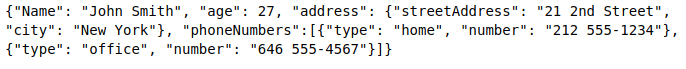
\includegraphics[width=1\textwidth,height=\textheight]{06_FileIO/json_example_compact.png}
\caption{JSON in compact form.}
\end{figure}

\note{Wikipedia (2019)}

\end{frame}

\begin{frame}[fragile,fragile]{}
\protect\hypertarget{section-4}{}

\begin{figure}
\centering
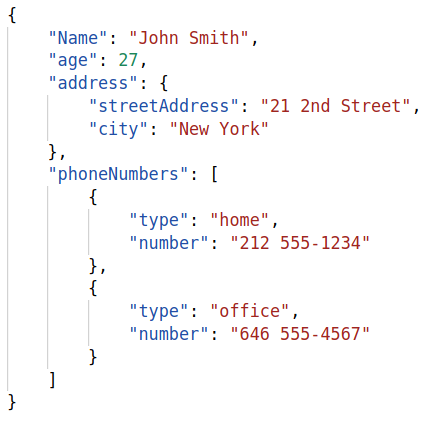
\includegraphics[width=0.65\textwidth,height=\textheight]{06_FileIO/json_example_long.png}
\caption{JSON indented.}
\end{figure}

\note{\begin{itemize}
\tightlist
\item
  unordered set of name:value pairs
\item
  begins with \texttt{\{} and ends with \texttt{\}}
\item
  name/value pairs are separated by \texttt{,}
\end{itemize}}

\end{frame}

\begin{frame}[fragile,fragile]{Tips for the Homework}
\protect\hypertarget{tips-for-the-homework}{}

\note{Make a plan for exercise 3.1

What steps do you need?

\begin{itemize}
\tightlist
\item
  collected ideas on the black board
\end{itemize}}

\end{frame}

\section*{References}
\addcontentsline{toc}{section}{References}

\begin{frame}{References}

\hypertarget{refs}{}
\leavevmode\hypertarget{ref-wiki:stream}{}%
Wikipedia. 2018. ``Stream (Computing) --- Wikipedia, the Free
Encyclopedia.''
\url{https://en.wikipedia.org/w/index.php?title=Stream_(computing)\&oldid=824727066}.

\leavevmode\hypertarget{ref-wiki:json}{}%
---------. 2019. ``JSON --- Wikipedia, the Free Encyclopedia.''
\url{https://en.wikipedia.org/w/index.php?title=JSON\&oldid=895923828}.

\end{frame}

\end{document}
